\documentclass[onesided]{article}\usepackage[]{graphicx}\usepackage[]{color}
% maxwidth is the original width if it is less than linewidth
% otherwise use linewidth (to make sure the graphics do not exceed the margin)
\makeatletter
\def\maxwidth{ %
  \ifdim\Gin@nat@width>\linewidth
    \linewidth
  \else
    \Gin@nat@width
  \fi
}
\makeatother

\definecolor{fgcolor}{rgb}{0.345, 0.345, 0.345}
\newcommand{\hlnum}[1]{\textcolor[rgb]{0.686,0.059,0.569}{#1}}%
\newcommand{\hlstr}[1]{\textcolor[rgb]{0.192,0.494,0.8}{#1}}%
\newcommand{\hlcom}[1]{\textcolor[rgb]{0.678,0.584,0.686}{\textit{#1}}}%
\newcommand{\hlopt}[1]{\textcolor[rgb]{0,0,0}{#1}}%
\newcommand{\hlstd}[1]{\textcolor[rgb]{0.345,0.345,0.345}{#1}}%
\newcommand{\hlkwa}[1]{\textcolor[rgb]{0.161,0.373,0.58}{\textbf{#1}}}%
\newcommand{\hlkwb}[1]{\textcolor[rgb]{0.69,0.353,0.396}{#1}}%
\newcommand{\hlkwc}[1]{\textcolor[rgb]{0.333,0.667,0.333}{#1}}%
\newcommand{\hlkwd}[1]{\textcolor[rgb]{0.737,0.353,0.396}{\textbf{#1}}}%
\let\hlipl\hlkwb

\usepackage{framed}
\makeatletter
\newenvironment{kframe}{%
 \def\at@end@of@kframe{}%
 \ifinner\ifhmode%
  \def\at@end@of@kframe{\end{minipage}}%
  \begin{minipage}{\columnwidth}%
 \fi\fi%
 \def\FrameCommand##1{\hskip\@totalleftmargin \hskip-\fboxsep
 \colorbox{shadecolor}{##1}\hskip-\fboxsep
     % There is no \\@totalrightmargin, so:
     \hskip-\linewidth \hskip-\@totalleftmargin \hskip\columnwidth}%
 \MakeFramed {\advance\hsize-\width
   \@totalleftmargin\z@ \linewidth\hsize
   \@setminipage}}%
 {\par\unskip\endMakeFramed%
 \at@end@of@kframe}
\makeatother

\definecolor{shadecolor}{rgb}{.97, .97, .97}
\definecolor{messagecolor}{rgb}{0, 0, 0}
\definecolor{warningcolor}{rgb}{1, 0, 1}
\definecolor{errorcolor}{rgb}{1, 0, 0}
\newenvironment{knitrout}{}{} % an empty environment to be redefined in TeX

\usepackage{alltt}
\usepackage[T1]{fontenc}
\linespread{1.5} % Line spacing - Palatino needs more space between lines
\usepackage{microtype} % Slightly tweak font spacing for aesthetics

\usepackage[hmarginratio=1:1,columnsep=20pt]{geometry} % Document margins
%\usepackage{multicol} % Used for the two-column layout of the document
\usepackage[hang, small,labelfont=bf,up,textfont=it,up]{caption} % Custom captions under/above floats in tables or figures
\usepackage{booktabs} % Horizontal rules in tables
\usepackage{float} % Required for tables and figures in the multi-column environment - they need to be placed in specific locations with the [H] (e.g. \begin{table}[H])

\usepackage{lettrine} % The lettrine is the first enlarged letter at the beginning of the text
\usepackage{paralist} % Used for the compactitem environment which makes bullet points with less space between them

% to ignore texts: good for thank messages and paper submissions.
      % \fbox{\phantom{This text will be invisible too, but a box will be printed arround it.}}

\usepackage{abstract} % Allows abstract customization
\renewcommand{\abstractnamefont}{\normalfont\bfseries} % Set the "Abstract" text to bold
%\renewcommand{\abstracttextfont}{\normalfont\small\itshape} % Set the abstract itself to small italic text

\usepackage[]{titlesec} % Allows customization of titles
\renewcommand\thesection{\Roman{section}} % Roman numerals for the sections
\renewcommand\thesubsection{\Roman{subsection}} % Roman numerals for subsections
\titleformat{\section}[block]{\large\scshape\centering}{\thesection.}{1em}{} % Change the look of the section titles
\titleformat{\subsection}[block]{\large}{\thesubsection.}{1em}{} % Change the look of the section titles

\usepackage{fancybox, fancyvrb, calc}
\usepackage[svgnames]{xcolor}
\usepackage{physics}
\usepackage{epigraph}
\usepackage{longtable}
\usepackage{pdflscape}
\usepackage{graphics}
\usepackage{pbox} % \pbox{20cm}{This is the first \\ cell}
\usepackage{amsfonts}
\usepackage{amsmath}
\usepackage{amssymb}
\usepackage{rotating}
\usepackage{paracol}
\usepackage{textcomp}
\usepackage[export]{adjustbox}
\usepackage{afterpage}
\usepackage{filecontents}
\usepackage{color}
\usepackage{latexsym}
\usepackage{lscape}       %\begin{landscape} and \end{landscape}
\usepackage{wasysym}
\usepackage{dashrule}
\usepackage{marvosym} % face package
\usepackage{framed}
\usepackage{tree-dvips}
\usepackage{pgffor}
\usepackage[]{authblk}
\usepackage{setspace}
\usepackage{array}
\usepackage[latin1]{inputenc}
\usepackage{hyperref}     %desactivar para link rojos
\usepackage{graphicx}
\usepackage{dcolumn} % for R tables
\usepackage{multirow} % For multirow in tables
\usepackage{pifont}
\usepackage{listings}




% hypothesis / theorem package begin
\usepackage{amsthm}
\usepackage{thmtools}
\declaretheoremstyle[
spaceabove=6pt, spacebelow=6pt,
headfont=\normalfont\bfseries,
notefont=\mdseries, notebraces={(}{)},
bodyfont=\normalfont,
postheadspace=0.6em,
headpunct=:
]{mystyle}
\declaretheorem[style=mystyle, name=Hypothesis, preheadhook={\renewcommand{\thehyp}{H\textsubscript{\arabic{hyp}}}}]{hyp}

\usepackage{cleveref}
\crefname{hyp}{hypothesis}{hypotheses}
\Crefname{hyp}{Hypothesis}{Hypotheses}
% hypothesis / theorem package end


%----------------------------------------------------------------------------------------
% Other ADDS-ON
%----------------------------------------------------------------------------------------

% independence symbol \independent
\newcommand\independent{\protect\mathpalette{\protect\independenT}{\perp}}
\def\independenT#1#2{\mathrel{\rlap{$#1#2$}\mkern2mu{#1#2}}}







\hypersetup{
    bookmarks=true,         % show bookmarks bar?
    unicode=false,          % non-Latin characters in Acrobat's bookmarks
    pdftoolbar=true,        % show Acrobat's toolbar?
    pdfmenubar=true,        % show Acrobat's menu?
    pdffitwindow=true,     % window fit to page when opened
    pdfstartview={FitH},    % fits the width of the page to the window
    pdftitle={My title},    % title
    pdfauthor={Author},     % author
    pdfsubject={Subject},   % subject of the document
    pdfcreator={Creator},   % creator of the document
    pdfproducer={Producer}, % producer of the document
    pdfkeywords={keyword1} {key2} {key3}, % list of keywords
    pdfnewwindow=true,      % links in new window
    colorlinks=true,       % false: boxed links; true: colored links
    linkcolor=ForestGreen,          % color of internal links (change box color with linkbordercolor)
    citecolor=ForestGreen,        % color of links to bibliography
    filecolor=ForestGreen,      % color of file links
    urlcolor=ForestGreen           % color of external links
}

%\usepackage[nodayofweek,level]{datetime} % to have date within text

\newcommand{\LETT}[3][]{\lettrine[lines=4,loversize=.2,#1]{\smash{#2}}{#3}} % letrine customization



% comments on margin
  % Select what to do with todonotes: 
  % \usepackage[disable]{todonotes} % notes not showed
  \usepackage[draft]{todonotes}   % notes showed
  % usage: \todo{This is a note at margin}

\usepackage{cooltooltips}

%%% bib begin
\usepackage[american]{babel}
\usepackage{csquotes}
\usepackage[backend=biber,style=authoryear,dashed=false,doi=false,isbn=false,url=false,arxiv=false]{biblatex}
%\DeclareLanguageMapping{american}{american-apa}
\addbibresource{/Users/hectorbahamonde/Bibliografia_PoliSci/library.bib} 
\addbibresource{/Users/hectorbahamonde/Bibliografia_PoliSci/Bahamonde_BibTex2013.bib} 

% USAGES
%% use \textcite to cite normal
%% \parencite to cite in parentheses
%% \footcite to cite in footnote
%% the default can be modified in autocite=FOO, footnote, for ex. 
%%% bib end

\usepackage{fancyhdr} % Headers and footers
\pagestyle{fancy} % All pages have headers and footers
\fancyhead{} % Blank out the default header
\fancyfoot{} % Blank out the default footer
\fancyhead[C]{MLE para Outcomes Binarios: Inferencia e Interpretaci\'on} % Custom header text
\fancyfoot[RO,LE]{\thepage} % Custom footer text
\IfFileExists{upquote.sty}{\usepackage{upquote}}{}
\begin{document}
% DOCUMENT ID
%----------------------------------------------------------------------------------------
%	CONTENT
%----------------------------------------------------------------------------------------

%\graphicspath{
%{/Users/hectorbahamonde/RU/Term5/Experiments_Redlawsk/Experiment/Data/}
%}



%%%%%%%%%%%%%%%%%%%%%%%%%%%%%%%%%%%%%%%%%%%%%%
% begin knitr stuff


%%%%%%%%%%%%%%%%%%%%%%%%%%%%%%%%%%%%%%%%%%%%%%





\hspace{-5mm}{\bf Profesor}: H\'ector Bahamonde, PhD.\\
\texttt{e:}\href{mailto:hector.bahamonde@uoh.cl}{\texttt{hector.bahamonde@uoh.cl}}\\
\texttt{w:}\href{http://www.hectorbahamonde.com}{\texttt{www.hectorbahamonde.com}}\\
{\bf Curso}: MLE.\\
\hspace{-5mm}{\bf TA}: Gonzalo Barr\'ia.

\section{Inferencia e Interpretaci\'on}

Los GLMs no se pueden interpretar usando la tabla. Los coeficientes no sifnifican lo que significaban en nuestro mundo OLS. Para interpretarlos, debemos usar otras herramientas. 


\paragraph{Intervalos de confianza}

Ya sabemos lo que un intervalo de confianza significa: si nuestra confianza es al 95\%, sabemos que el ``true value'' de la estimaci\'on caer\'a el 95\% dentro del margen de los intervalos de confianza. Es en base a esto que antes hablabamos de ``significancia estad\'istica''.

Carguemos los datos


\begin{knitrout}
\definecolor{shadecolor}{rgb}{0.969, 0.969, 0.969}\color{fgcolor}\begin{kframe}
\begin{alltt}
\hlcom{# Data}
\hlstd{mydata} \hlkwb{<-} \hlkwd{read.csv}\hlstd{(}\hlstr{"https://stats.idre.ucla.edu/stat/data/binary.csv"}\hlstd{)}
\hlkwd{head}\hlstd{(mydata)}
\end{alltt}
\begin{verbatim}
##   admit gre  gpa rank
## 1     0 380 3.61    3
## 2     1 660 3.67    3
## 3     1 800 4.00    1
## 4     1 640 3.19    4
## 5     0 520 2.93    4
## 6     1 760 3.00    2
\end{verbatim}
\begin{alltt}
\hlkwd{summary}\hlstd{(mydata)}
\end{alltt}
\begin{verbatim}
##      admit             gre             gpa             rank      
##  Min.   :0.0000   Min.   :220.0   Min.   :2.260   Min.   :1.000  
##  1st Qu.:0.0000   1st Qu.:520.0   1st Qu.:3.130   1st Qu.:2.000  
##  Median :0.0000   Median :580.0   Median :3.395   Median :2.000  
##  Mean   :0.3175   Mean   :587.7   Mean   :3.390   Mean   :2.485  
##  3rd Qu.:1.0000   3rd Qu.:660.0   3rd Qu.:3.670   3rd Qu.:3.000  
##  Max.   :1.0000   Max.   :800.0   Max.   :4.000   Max.   :4.000
\end{verbatim}
\end{kframe}
\end{knitrout}

Estimemos el primer modelo

\begin{knitrout}
\definecolor{shadecolor}{rgb}{0.969, 0.969, 0.969}\color{fgcolor}\begin{kframe}
\begin{alltt}
\hlstd{logit.1} \hlkwb{<-} \hlkwd{glm}\hlstd{(admit} \hlopt{~} \hlstd{gre} \hlopt{+} \hlstd{gpa,} \hlkwc{data} \hlstd{= mydata,} \hlkwc{family} \hlstd{=} \hlkwd{binomial}\hlstd{(}\hlkwc{link} \hlstd{=} \hlstr{"logit"}\hlstd{))}
\hlkwd{summary}\hlstd{(logit.1)}
\end{alltt}
\begin{verbatim}
## 
## Call:
## glm(formula = admit ~ gre + gpa, family = binomial(link = "logit"), 
##     data = mydata)
## 
## Deviance Residuals: 
##     Min       1Q   Median       3Q      Max  
## -1.2730  -0.8988  -0.7206   1.3013   2.0620  
## 
## Coefficients:
##              Estimate Std. Error z value   Pr(>|z|)    
## (Intercept) -4.949378   1.075093  -4.604 0.00000415 ***
## gre          0.002691   0.001057   2.544     0.0109 *  
## gpa          0.754687   0.319586   2.361     0.0182 *  
## ---
## Signif. codes:  0 '***' 0.001 '**' 0.01 '*' 0.05 '.' 0.1 ' ' 1
## 
## (Dispersion parameter for binomial family taken to be 1)
## 
##     Null deviance: 499.98  on 399  degrees of freedom
## Residual deviance: 480.34  on 397  degrees of freedom
## AIC: 486.34
## 
## Number of Fisher Scoring iterations: 4
\end{verbatim}
\end{kframe}
\end{knitrout}

Y ahora, estimemos los intervalos de confianza. Los intervalos de confianza son sencillos de calcular. Si queremos un 95\% de confianza, miramos la tabla con los valores Z. Para ese porcentaje es $1.960$ (para un 90\% es 1.645). 

\begin{equation}
\hat\theta \pm 1.960 \times \text{SE}_{\hat\theta}
\end{equation}

donde $\hat\theta$ es la estimaci\'on (el par\'ametro), $1.960$ es el valor $z$, DS es la desviaci\'on est\'andard, y N es el largo de la base de datos. Si te fijas, tenemos el signo $\pm$ que implica que debemos restar para obtener el rango m\'inimo del intervalo de confianza, y sumar para obtener el rango m\'aximo del intervalo de confianza.

Por ejemplo, el coeficiente de ``gre'' es $\hat\theta=0.0026907$, el $SE = 0.001094$. Entonces, $0.002264426 + 1.96*0.001094$ para el intervalo superior, y $0.002264426 - 1.96*0.001094$ para el intervalo inferior. 

Usemos un paquete.



\begin{knitrout}
\definecolor{shadecolor}{rgb}{0.969, 0.969, 0.969}\color{fgcolor}\begin{kframe}
\begin{alltt}
\hlkwd{confint}\hlstd{(logit.1)}
\end{alltt}
\begin{verbatim}
##                     2.5 %       97.5 %
## (Intercept) -7.1092205752 -2.886726963
## gre          0.0006373958  0.004791712
## gpa          0.1347509288  1.390131131
\end{verbatim}
\end{kframe}
\end{knitrout}


\paragraph{Odds Ratios}

Esta manera de interpretar solo funciona con los \emph{link function} tipo logit (logit, multinomial logit, etc.), no probit links (i.e. probit, multinomial probit). Formalmente, 

\begin{equation}\label{odd:ratio}
\begin{split}
ln \Omega(\text{x}) & = \text{x}\beta \\
\Omega(\text{x}) & = \frac{\text{Pr}(\text{y}=1 | \text{x})}{\text{Pr}(\text{y}=0 | \text{x})} 
\end{split}
\end{equation}

donde \autoref{odd:ratio} es el \emph{odd ratio} de que $y$ sea 1 dado $x$, relativo a que $y$ sea 0 dado $x$. Es un ratio, una fracci\'on. Su interpretaci\'on es intuititiva: ``cuando $x$ cambia, cu\'anto cambia el logit estimado ($\hat\theta$) manteniendo los otros parametros constantes''?

{\bf Lo bueno} de esta interpretacion es que podemos observar el cambio de la variable dependiente. Ten en cuenta que los \emph{odds ratios} son comparables s\'olo con la misma variable. {\bf Lo malo} es que seguimos en unidades de la escala logit (que sigue siendo poco interpretable).



\begin{knitrout}
\definecolor{shadecolor}{rgb}{0.969, 0.969, 0.969}\color{fgcolor}\begin{kframe}
\begin{alltt}
\hlkwd{p_load}\hlstd{(oddsratio)}
\hlcom{#}
\hlkwd{or_glm}\hlstd{(}\hlkwc{data} \hlstd{= mydata,}
       \hlkwc{model} \hlstd{= logit.1,}
       \hlkwc{incr} \hlstd{=} \hlkwd{list}\hlstd{(}\hlkwc{gre} \hlstd{=} \hlnum{380}\hlstd{,} \hlkwc{gpa} \hlstd{=} \hlnum{5}\hlstd{))}
\end{alltt}
\begin{verbatim}
##   predictor oddsratio ci_low (2.5) ci_high (97.5) increment
## 1       gre     2.780        1.274          6.177       380
## 2       gpa    43.529        1.962       1043.834         5
\end{verbatim}
\end{kframe}
\end{knitrout}

Aqu\'i vemos que la variable dependiente (\texttt{admit}) es 55 veces m\'as probable de ocurrir cuando la variable independiente \texttt{gpa} incrementa de su media (3.3899) a 5. Como ves, ganamos interpretatibilidad del modelo. 

\begin{knitrout}
\definecolor{shadecolor}{rgb}{0.969, 0.969, 0.969}\color{fgcolor}\begin{kframe}
\begin{alltt}
\hlkwd{par}\hlstd{(}\hlkwc{mfrow}\hlstd{=}\hlkwd{c}\hlstd{(}\hlnum{1}\hlstd{,}\hlnum{2}\hlstd{))}
\hlkwd{hist}\hlstd{(mydata}\hlopt{$}\hlstd{gpa,} \hlkwc{main} \hlstd{=} \hlstr{"GPA"}\hlstd{)}
\hlkwd{hist}\hlstd{(mydata}\hlopt{$}\hlstd{gre,} \hlkwc{main} \hlstd{=} \hlstr{"GRE"}\hlstd{)}
\end{alltt}
\end{kframe}

{\centering 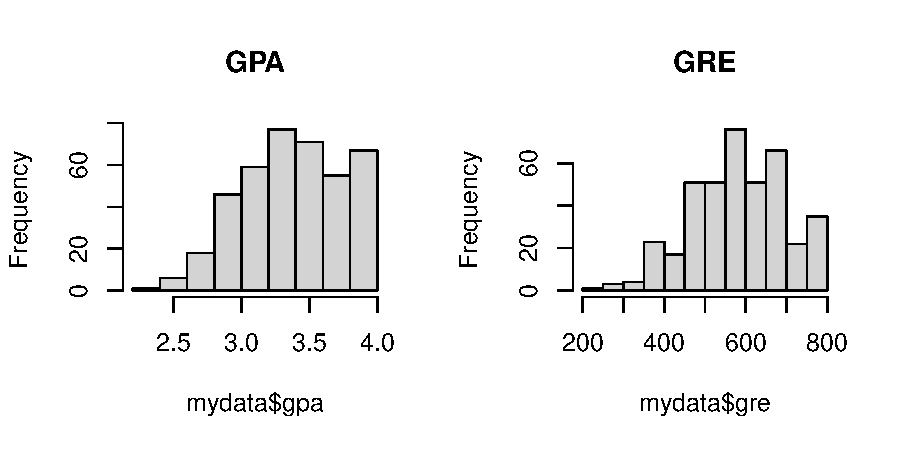
\includegraphics[width=\maxwidth]{figure/od:plot-1} 

}



\end{knitrout}

Como interpretamos \texttt{GRE}?

\begin{knitrout}
\definecolor{shadecolor}{rgb}{0.969, 0.969, 0.969}\color{fgcolor}\begin{kframe}
\begin{alltt}
\hlkwd{mean}\hlstd{(mydata}\hlopt{$}\hlstd{gpa)}
\end{alltt}
\begin{verbatim}
## [1] 3.3899
\end{verbatim}
\begin{alltt}
\hlkwd{mean}\hlstd{(mydata}\hlopt{$}\hlstd{gre)}
\end{alltt}
\begin{verbatim}
## [1] 587.7
\end{verbatim}
\end{kframe}
\end{knitrout}

Si bien es cierto que ganamos interpretaci\'on del modelo, lo malo es seguimos hablando con poca precisi\'on. Decir que algo es 55 veces m\'as probable es interesante, pero no s\'e si tan ``cient\'ifico''.


\paragraph{\emph{Partial/Marginal Changes} in y}

Los ``cambios parciales'' son muy parecidos a los \emph{odds ratios}. Son parecidos porque nos muestra ``cuando cambia $\hat y$ cuando cambia $x$''. Formalmente, 

\begin{equation}\label{part:chan}
\frac{\partial \hat y}{\partial x_{k}} = \beta_{k}
\end{equation}

lo que significa ``por un cambio en $x_{k}$, se espera que $\hat y$ cambie $\beta_{k}$'' (manteniendo todas las otras variables constantes en su media). Sin embargo, debido a que la varianza de $\hat y$ es desconocida (la varianza es un \emph{population parameter}), entonces, esto complica la interpretacion de $\beta_{k}$. Para resolver esto, lo que hacemos es pensar en coeficientes $\beta_{k}$ estandarizados. Siguiendo \autoref{part:chan}, lo que pensamos es en ``por un cambio en $x_{k}$, se espera que $\hat y$ cambie $\beta_{k}$ {\bf desviaciones est\'andard}''. Formalmente, 

\begin{equation}\label{part:chan}
\beta_{k}^{S} = \frac{\sigma_{k} \beta_{k}}{\sigma_{\hat y}} = \sigma_{k}\beta_{k}^{S_{\hat y}}
\end{equation}

Nota que \label{part:chan} tambi\'en estandariza $\hat y$. Debido a que $\hat\sigma_{\hat y} = \sigma_{\hat y}$ (i.e. podemos estimar la varianza estandarizada de los datos), 

\begin{equation}%\label{part:chan}
{\hat\sigma_{\hat y}} = \beta^{\top}\hat\sigma(x)\beta + \sigma(\epsilon)
\end{equation}

Calculemos dos escenarios. Uno donde el estudiante le iba muy mal en el colegio, pero tuvo un buen puntaje en la prueba de admisi\'on de doctorado (GRE).

\begin{knitrout}
\definecolor{shadecolor}{rgb}{0.969, 0.969, 0.969}\color{fgcolor}\begin{kframe}
\begin{alltt}
\hlkwd{p_load}\hlstd{(margins)}
\hlkwd{summary}\hlstd{(}\hlkwd{margins}\hlstd{(logit.1,}
        \hlkwc{at} \hlstd{=} \hlkwd{list}\hlstd{(}
          \hlkwc{gre} \hlstd{=} \hlkwd{min}\hlstd{(mydata}\hlopt{$}\hlstd{gre),}
          \hlkwc{gpa} \hlstd{=} \hlkwd{max}\hlstd{(mydata}\hlopt{$}\hlstd{gpa))}
        \hlstd{))}
\end{alltt}
\begin{verbatim}
##  factor      gre    gpa    AME     SE      z      p   lower  upper
##     gpa 220.0000 4.0000 0.1242 0.0808 1.5364 0.1244 -0.0342 0.2827
##     gre 220.0000 4.0000 0.0004 0.0001 5.9659 0.0000  0.0003 0.0006
\end{verbatim}
\end{kframe}
\end{knitrout}

Ahora calculemos el opuesto:

\begin{knitrout}
\definecolor{shadecolor}{rgb}{0.969, 0.969, 0.969}\color{fgcolor}\begin{kframe}
\begin{alltt}
\hlkwd{summary}\hlstd{(}\hlkwd{margins}\hlstd{(logit.1,}
        \hlkwc{at} \hlstd{=} \hlkwd{list}\hlstd{(}
          \hlkwc{gre} \hlstd{=} \hlkwd{max}\hlstd{(mydata}\hlopt{$}\hlstd{gre),}
          \hlkwc{gpa} \hlstd{=} \hlkwd{min}\hlstd{(mydata}\hlopt{$}\hlstd{gpa)}\hlopt{:}\hlkwd{mean}\hlstd{(mydata}\hlopt{$}\hlstd{gpa))}
          \hlstd{))}
\end{alltt}
\begin{verbatim}
##  factor      gre    gpa    AME     SE      z      p   lower  upper
##     gpa 800.0000 2.2600 0.1420 0.0325 4.3633 0.0000  0.0782 0.2058
##     gpa 800.0000 3.2600 0.1834 0.0741 2.4771 0.0132  0.0383 0.3286
##     gre 800.0000 2.2600 0.0005 0.0003 1.6967 0.0898 -0.0001 0.0011
##     gre 800.0000 3.2600 0.0007 0.0003 2.3188 0.0204  0.0001 0.0012
\end{verbatim}
\end{kframe}
\end{knitrout}

Para entender mejor esto, grafiquemos:

\begin{knitrout}
\definecolor{shadecolor}{rgb}{0.969, 0.969, 0.969}\color{fgcolor}\begin{kframe}
\begin{alltt}
\hlkwd{par}\hlstd{(}\hlkwc{mfrow}\hlstd{=}\hlkwd{c}\hlstd{(}\hlnum{1}\hlstd{,}\hlnum{2}\hlstd{))}
\hlkwd{cplot}\hlstd{(logit.1,} \hlstr{"gre"}\hlstd{)}
\end{alltt}
\begin{verbatim}
##       xvals     yvals     upper      lower
## 1  220.0000 0.1419589 0.2412899 0.04262786
## 2  244.1667 0.1500652 0.2479355 0.05219492
## 3  268.3333 0.1585489 0.2545321 0.06256566
## 4  292.5000 0.1674177 0.2610725 0.07376288
## 5  316.6667 0.1766785 0.2675539 0.08580299
## 6  340.8333 0.1863368 0.2739798 0.09869393
## 7  365.0000 0.1963973 0.2803622 0.11243234
## 8  389.1667 0.2068628 0.2867259 0.12699962
## 9  413.3333 0.2177348 0.2931134 0.14235622
## 10 437.5000 0.2290133 0.2995933 0.15843330
## 11 461.6667 0.2406962 0.3062725 0.17512003
## 12 485.8333 0.2527798 0.3133146 0.19224490
## 13 510.0000 0.2652580 0.3209666 0.20954944
## 14 534.1667 0.2781229 0.3295882 0.22665765
## 15 558.3333 0.2913644 0.3396690 0.24305980
## 16 582.5000 0.3049699 0.3517828 0.25815704
## 17 606.6667 0.3189249 0.3664325 0.27141726
## 18 630.8333 0.3332122 0.3838358 0.28258868
## 19 655.0000 0.3478128 0.4038425 0.29178301
## 20 679.1667 0.3627051 0.4260603 0.29934986
\end{verbatim}
\begin{alltt}
\hlkwd{cplot}\hlstd{(logit.1,} \hlstr{"gpa"}\hlstd{)}
\end{alltt}
\begin{verbatim}
##     xvals     yvals     upper      lower
## 1  2.2600 0.1594306 0.2615309 0.05733021
## 2  2.3325 0.1669004 0.2668014 0.06699931
## 3  2.4050 0.1746474 0.2719973 0.07729752
## 4  2.4775 0.1826752 0.2771187 0.08823181
## 5  2.5500 0.1909867 0.2821696 0.09980371
## 6  2.6225 0.1995839 0.2871600 0.11200782
## 7  2.6950 0.2084684 0.2921072 0.12482964
## 8  2.7675 0.2176409 0.2970392 0.13824262
## 9  2.8400 0.2271012 0.3019984 0.15220395
## 10 2.9125 0.2368481 0.3070478 0.16664844
## 11 2.9850 0.2468798 0.3122801 0.18147962
## 12 3.0575 0.2571932 0.3178294 0.19655702
## 13 3.1300 0.2677843 0.3238891 0.21167944
## 14 3.2025 0.2786478 0.3307294 0.22656631
## 15 3.2750 0.2897777 0.3387074 0.24084799
## 16 3.3475 0.3011665 0.3482440 0.25408903
## 17 3.4200 0.3128058 0.3597384 0.26587323
## 18 3.4925 0.3246859 0.3734345 0.27593734
## 19 3.5650 0.3367961 0.3893290 0.28426321
## 20 3.6375 0.3491245 0.4072024 0.29104653
\end{verbatim}
\end{kframe}

{\centering 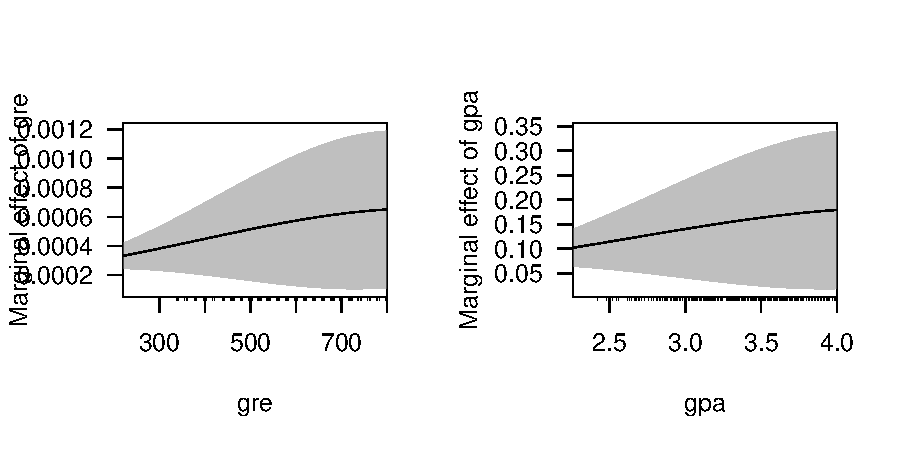
\includegraphics[width=\maxwidth]{figure/sc3-1} 

}



\end{knitrout}


\paragraph{Predicted Probabilities: Gr\'aficos}

Quiz\'as esta sea la manera m\'as usada para poder interpretar: graficando (o mostrando en una tabla) ``la probabilidad de que $y$ sea $1$ a distintos valores de $x$'', o de manera m\'as formal, 

\begin{equation}%\label{part:chan}
\hat{\text{Pr}}(y_{i}=1|{\mathbf x}_{i}) = f({\mathbf x}_{i}\hat{\mathbf \beta})
\end{equation}

F\'ijate que ${\mathbf x}$ y $\hat{\mathbf \beta}$ son matrices. {\color{red}Por que?} 

Aqui lo que queremos saber es como se comparta la probabilidad de que $y_{i}=1$ a medida que nos movemos en una de las $x$'s. {\bf Lo bueno}, es que tenemos un lenguaje f\'acil de entender: todos entienden probabilidades, y adem\'as, estas var\'ian entre 0 y 1. {\color{red}Pero qu\'e hacemos con el resto de las x's?}

Para predecir usaremos el comando \texttt{predict}


\begin{knitrout}
\definecolor{shadecolor}{rgb}{0.969, 0.969, 0.969}\color{fgcolor}\begin{kframe}
\begin{alltt}
\hlkwd{head}\hlstd{(}\hlkwd{predict}\hlstd{(logit.1))}
\end{alltt}
\begin{verbatim}
##          1          2          3          4          5          6 
## -1.2024987 -0.4038261  0.2219162 -0.8198895 -1.3389901 -0.6403980
\end{verbatim}
\begin{alltt}
\hlkwd{plot}\hlstd{(}\hlkwd{predict}\hlstd{(logit.1))} \hlcom{# logit scale}
\end{alltt}
\end{kframe}

{\centering 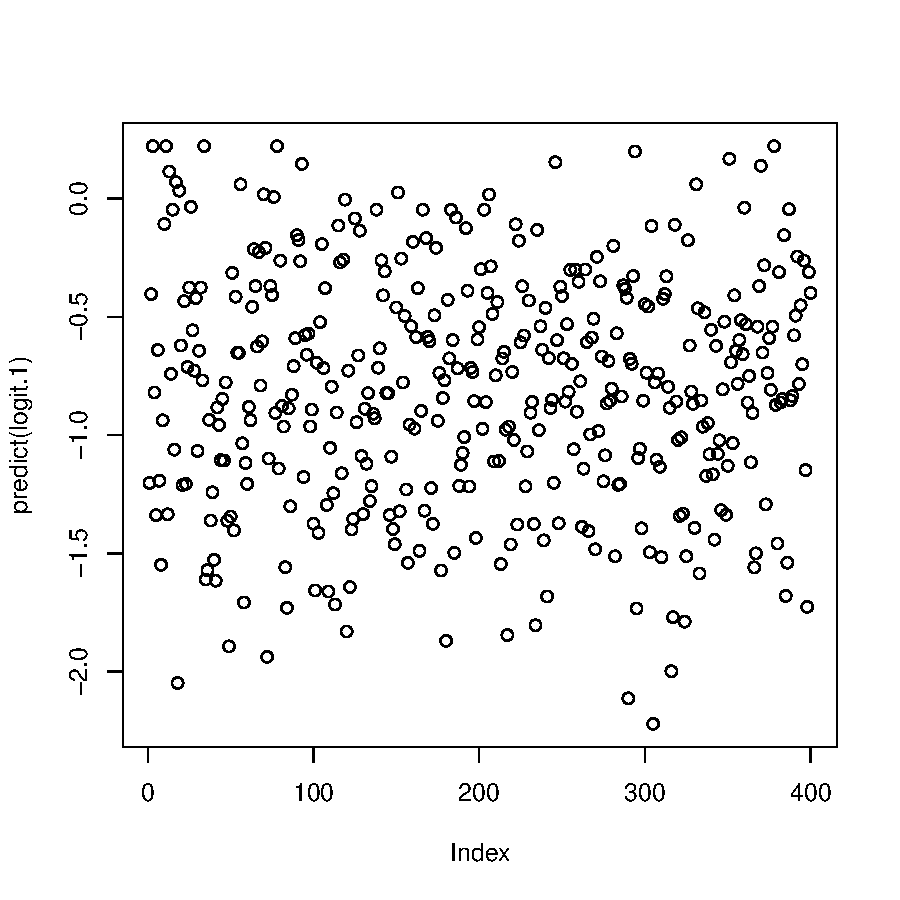
\includegraphics[width=\maxwidth]{figure/predict:1-1} 

}


\begin{kframe}\begin{alltt}
\hlkwd{plot}\hlstd{(}\hlkwd{predict}\hlstd{(logit.1,} \hlkwc{type}\hlstd{=}\hlstr{"response"}\hlstd{))} \hlcom{# Predicted Prob}
\end{alltt}
\end{kframe}

{\centering 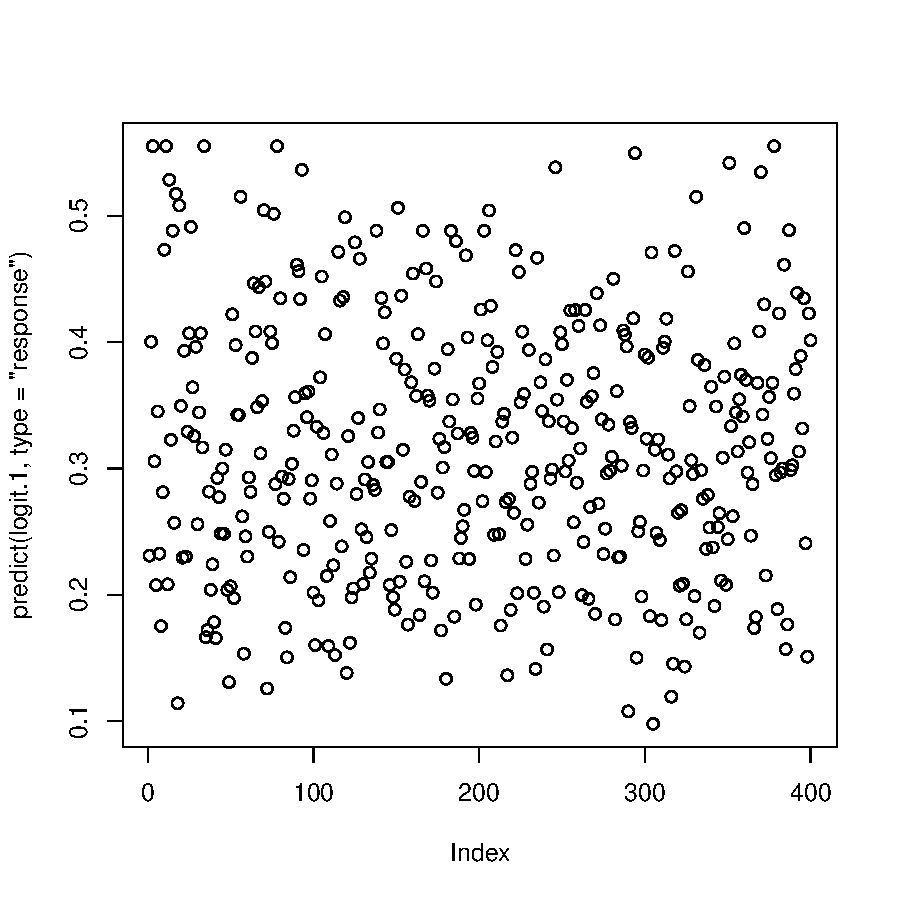
\includegraphics[width=\maxwidth]{figure/predict:1-2} 

}



\end{knitrout}

Usando la librer\'ia \texttt{effects}, podremos graficar. 


\begin{knitrout}
\definecolor{shadecolor}{rgb}{0.969, 0.969, 0.969}\color{fgcolor}\begin{kframe}
\begin{alltt}
\hlkwd{p_load}\hlstd{(}\hlstr{"effects"}\hlstd{)}
\hlkwd{par}\hlstd{(}\hlkwc{mfrow}\hlstd{=}\hlkwd{c}\hlstd{(}\hlnum{1}\hlstd{,}\hlnum{1}\hlstd{))}
\hlkwd{plot}\hlstd{(}\hlkwd{predictorEffects}\hlstd{(logit.1))} \hlcom{# Todo el modelo (PLURAL)}
\end{alltt}
\end{kframe}

{\centering 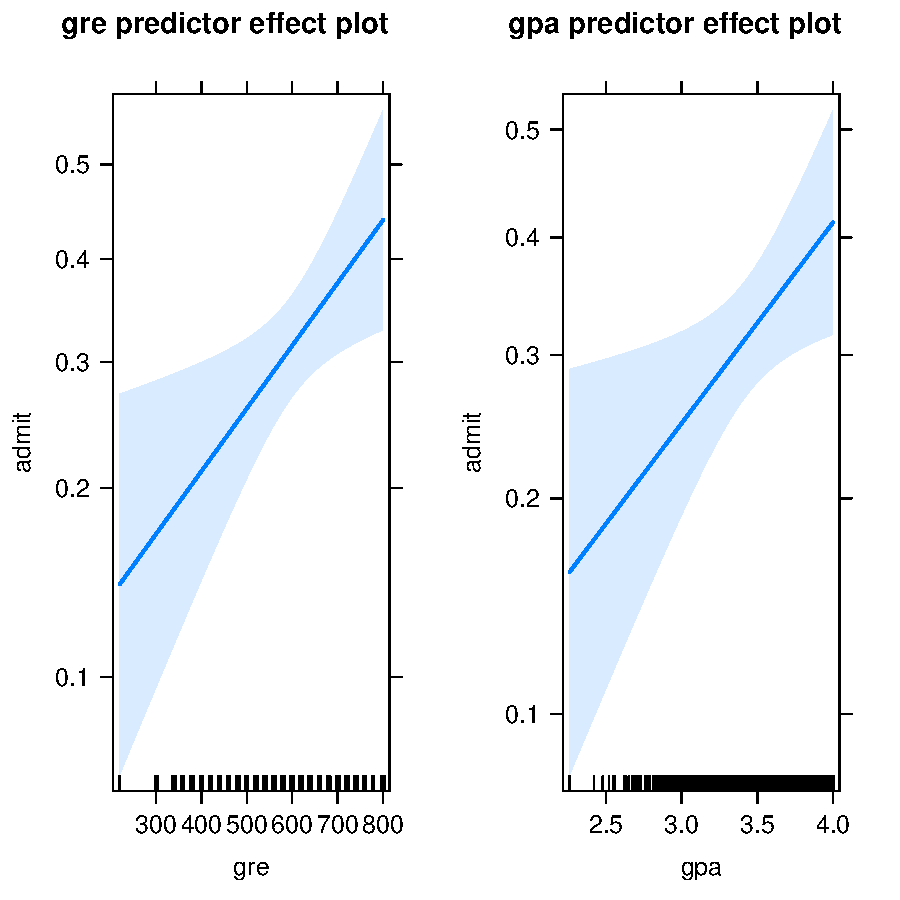
\includegraphics[width=\maxwidth]{figure/predict:2-1} 

}


\begin{kframe}\begin{alltt}
\hlkwd{par}\hlstd{(}\hlkwc{mfrow}\hlstd{=}\hlkwd{c}\hlstd{(}\hlnum{1}\hlstd{,}\hlnum{2}\hlstd{))}
\hlkwd{plot}\hlstd{(}\hlkwd{predictorEffect}\hlstd{(}\hlstr{"gre"}\hlstd{, logit.1))} \hlcom{# Solo una variable (SINGULAR)}
\end{alltt}
\end{kframe}

{\centering 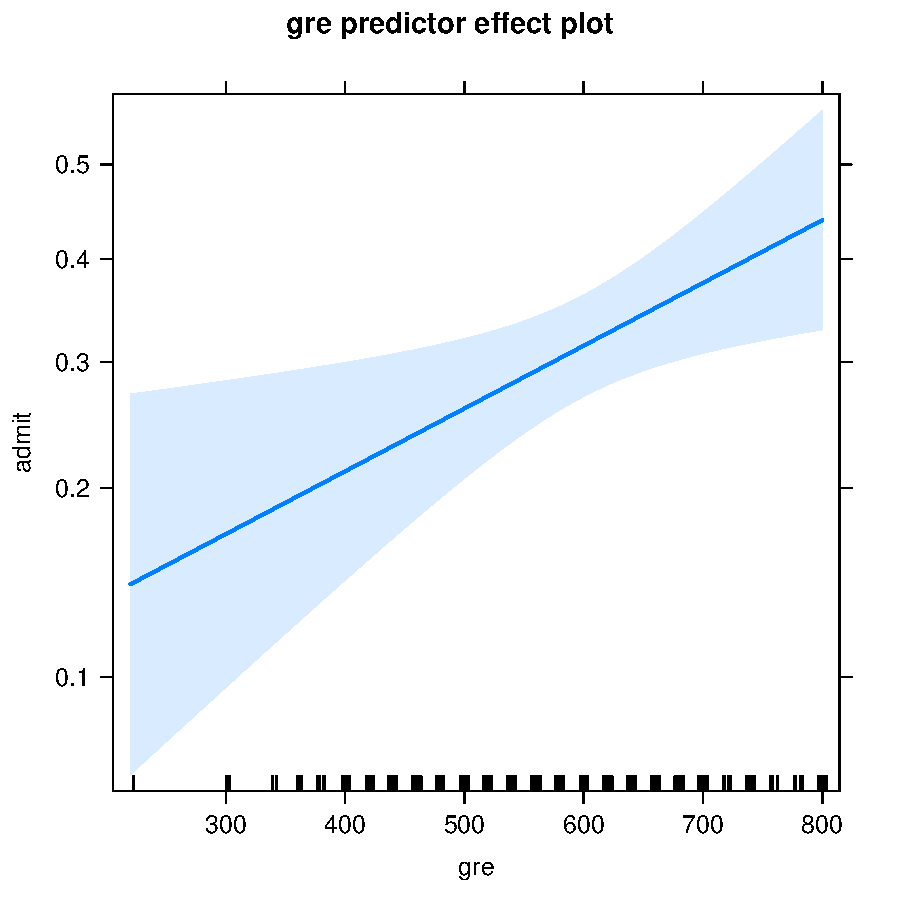
\includegraphics[width=\maxwidth]{figure/predict:2-2} 

}


\begin{kframe}\begin{alltt}
\hlkwd{plot}\hlstd{(gpa.pred.prob} \hlkwb{<-} \hlkwd{predictorEffect}\hlstd{(}\hlstr{"gpa"}\hlstd{, logit.1))} \hlcom{# Solo una variable (SINGULAR)}
\end{alltt}
\end{kframe}

{\centering 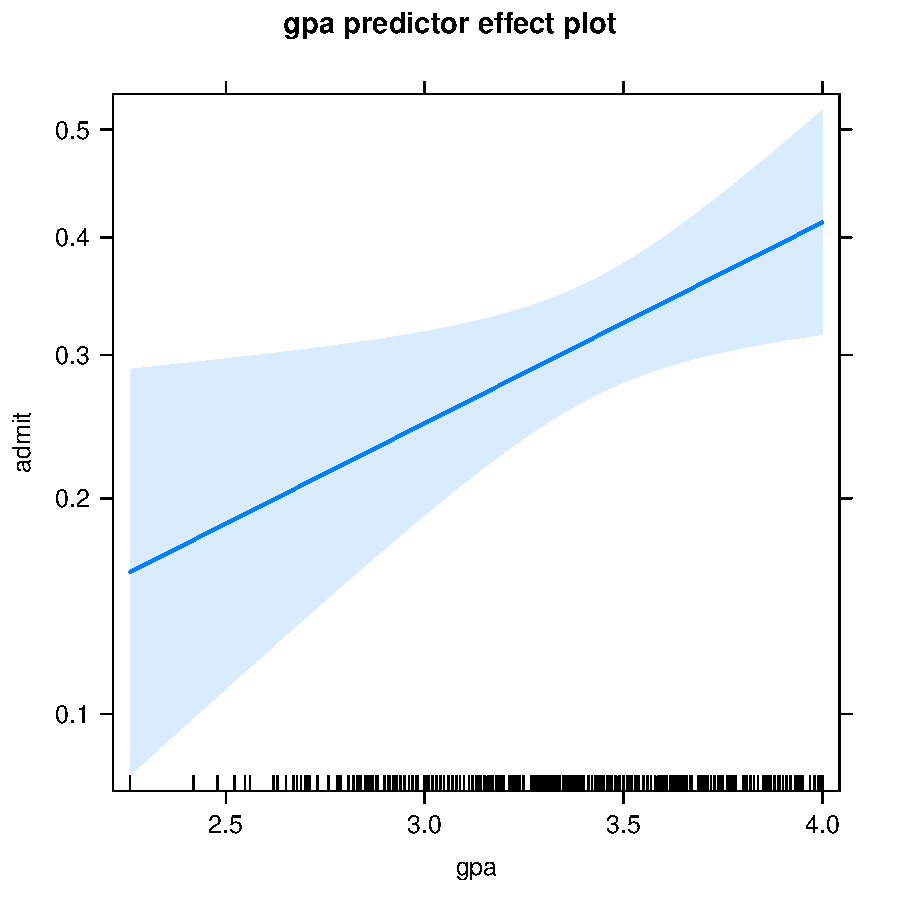
\includegraphics[width=\maxwidth]{figure/predict:2-3} 

}



\end{knitrout}



\paragraph{Predicted Probabilities: Tablas}

La otra alternativa es poder generar tablas con \emph{predicted prob's}. La idea es ir generando ``perfiles'' que hagan sentido desde un punto de vista substantivo. 

\begin{knitrout}
\definecolor{shadecolor}{rgb}{0.969, 0.969, 0.969}\color{fgcolor}\begin{kframe}
\begin{alltt}
\hlcom{# generar los rangos de los perfiles deseados}
\hlstd{gpa.bajo} \hlkwb{<-} \hlkwd{with}\hlstd{(mydata,}
                \hlkwd{data.frame}\hlstd{(}
                        \hlkwc{gre} \hlstd{=} \hlkwd{c}\hlstd{(}\hlkwd{min}\hlstd{(mydata}\hlopt{$}\hlstd{gre),} \hlkwd{max}\hlstd{(mydata}\hlopt{$}\hlstd{gre)),}
                        \hlkwc{gpa} \hlstd{=} \hlkwd{min}\hlstd{(mydata}\hlopt{$}\hlstd{gpa))}
                \hlstd{)}
\hlstd{gpa.medio} \hlkwb{<-} \hlkwd{with}\hlstd{(mydata,}
                 \hlkwd{data.frame}\hlstd{(}
                         \hlkwc{gre} \hlstd{=} \hlkwd{c}\hlstd{(}\hlkwd{min}\hlstd{(mydata}\hlopt{$}\hlstd{gre),} \hlkwd{max}\hlstd{(mydata}\hlopt{$}\hlstd{gre)),}
                         \hlkwc{gpa} \hlstd{=} \hlkwd{mean}\hlstd{(mydata}\hlopt{$}\hlstd{gpa,} \hlkwc{na.rm} \hlstd{= T))}
                         \hlstd{)}
\hlstd{gpa.alto} \hlkwb{<-} \hlkwd{with}\hlstd{(mydata,}
                      \hlkwd{data.frame}\hlstd{(}
                              \hlkwc{gre} \hlstd{=} \hlkwd{c}\hlstd{(}\hlkwd{min}\hlstd{(mydata}\hlopt{$}\hlstd{gre),} \hlkwd{max}\hlstd{(mydata}\hlopt{$}\hlstd{gre)),}
                              \hlkwc{gpa} \hlstd{=} \hlkwd{max}\hlstd{(mydata}\hlopt{$}\hlstd{gpa))}
                              \hlstd{)}
\end{alltt}
\end{kframe}
\end{knitrout}


\begin{knitrout}
\definecolor{shadecolor}{rgb}{0.969, 0.969, 0.969}\color{fgcolor}\begin{kframe}
\begin{alltt}
\hlcom{# usar funcion predict}
\hlkwd{predict}\hlstd{(logit.1, gpa.bajo,} \hlkwc{type}\hlstd{=}\hlstr{"response"}\hlstd{)}
\end{alltt}
\begin{verbatim}
##          1          2 
## 0.06587598 0.25138506
\end{verbatim}
\begin{alltt}
\hlkwd{predict}\hlstd{(logit.1, gpa.medio,} \hlkwc{type}\hlstd{=}\hlstr{"response"}\hlstd{)}
\end{alltt}
\begin{verbatim}
##         1         2 
## 0.1419589 0.4406515
\end{verbatim}
\begin{alltt}
\hlkwd{predict}\hlstd{(logit.1, gpa.alto,} \hlkwc{type}\hlstd{=}\hlstr{"response"}\hlstd{)}
\end{alltt}
\begin{verbatim}
##         1         2 
## 0.2077272 0.5552525
\end{verbatim}
\end{kframe}
\end{knitrout}



\begin{table}[H]
\begin{tabular}{|c|c|c|c|c|c|}
\hline
\multicolumn{2}{|c|}{\textbf{GPA Bajo}} & \multicolumn{2}{c|}{\textbf{GPA Medio}} & \multicolumn{2}{c|}{\textbf{GPA Alto}} \\ \hline
\textit{Gre Min}   & \textit{Gre Max}   & \textit{Gre Min}   & \textit{Gre Max}   & \textit{Gre Min}   & \textit{Gre Max}  \\ \hline
0.07 & 0.25 &                    
0.14 & 0.44 &                    
0.21 & 0.56 \\ \hline
\end{tabular}
\end{table}


{\color{red}Cu\'al es el problema?}

\begin{knitrout}
\definecolor{shadecolor}{rgb}{0.969, 0.969, 0.969}\color{fgcolor}\begin{kframe}
\begin{alltt}
\hlstd{knitr}\hlopt{::}\hlkwd{purl}\hlstd{(}\hlstr{'Inferencia_Interpretacion.Rnw'}\hlstd{)}
\end{alltt}


{\ttfamily\noindent\bfseries\color{errorcolor}{\#\# Error in parse\_block(g[-1], g[1], params.src, markdown\_mode): Duplicate chunk label 'setup20', which has been used for the chunk:\\\#\# if (!require("{}pacman"{})) install.packages("{}pacman"{}); library(pacman)\\\#\# p\_load(knitr)\\\#\# set.seed(2020)\\\#\# options(scipen=9999999)}}\begin{alltt}
\hlkwd{Stangle}\hlstd{(}\hlstr{'Inferencia_Interpretacion.Rnw'}\hlstd{)}
\end{alltt}
\begin{verbatim}
## Writing to file Inferencia_Interpretacion.R
\end{verbatim}
\end{kframe}
\end{knitrout}

%\newpage
%\paragraph{}
%\paragraph{}
%\pagenumbering{Roman}
%\setcounter{page}{1}
%\printbibliography



\end{document}


